\documentclass[handout]{beamer}
\mode<presentation>{}
\usetheme{Dresden}
\usepackage{apalike}
\usepackage{graphicx}
\usepackage{subcaption}
\usepackage{movie15}
\usepackage{mwe,tikz}\usepackage[percent]{overpic}
%% preamble
\title{Water and Dispersive Shocks}
\author{Jordan Pitt, Stephen Roberts and Christopher Zoppou \\ Australian National University}
\newcommand\solidrule[1][0.25cm]{\rule[0.5ex]{#1}{1pt}}
\newcommand\dashedrule{\mbox{\solidrule[2mm]\hspace{2mm}\solidrule[2mm]}}
\newcommand{\dotrule}[1]{%
	\parbox[]{#1}{\dotfill}}

\begin{document}
%% title frame
\begin{frame}
\titlepage
\end{frame}
\begin{frame}{Outline}
	\begin{itemize}
		\item Motivation: Water \pause
		\item Nonlinear Shocks: Shallow Water Wave Equations \pause
		\item Dispersive Shocks: Serre Equations
	\end{itemize}
\end{frame}
%% normal frame
\section{Water and Shocks}
\begin{frame}{Water}
\begin{figure}
	\centering
	\begin{subfigure}{0.5\textwidth}
		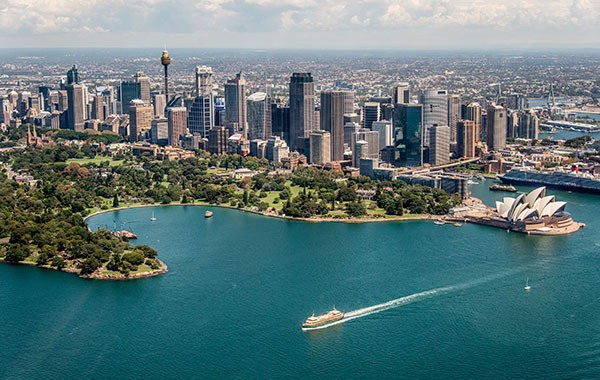
\includegraphics[width=0.9\textwidth]{./Figures/SydneyHarbour.jpg}
		\subcaption{Sydney Harbour}
		\vspace{0.5cm}
	\end{subfigure}%
	\pause
	\begin{subfigure}{0.475\textwidth}
		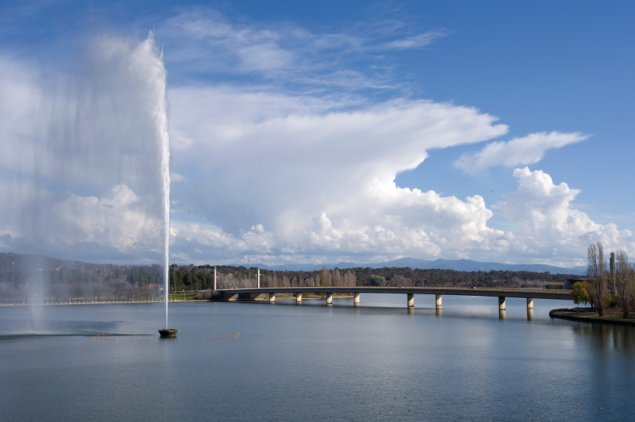
\includegraphics[width=0.9\textwidth]{./Figures/LakeBG.jpg}
		\subcaption{Lake Burley Griffin}
		\vspace{0.5cm}
	\end{subfigure}
		\end{figure}
\end{frame}

\begin{frame}{Waves}
\begin{figure}
	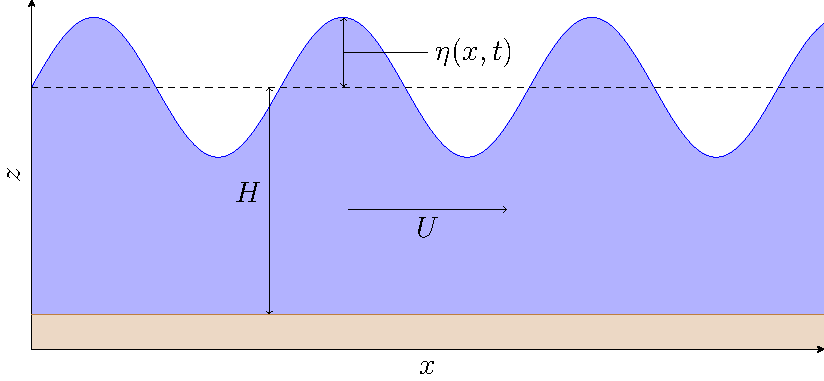
\includegraphics[width=\textwidth]{./Figures/Latex/Wavetank.pdf}
\end{figure}	
\end{frame}

\begin{frame}{Linear Wave Speed}
\begin{equation*}
v_p = U \pm\sqrt{\frac{g}{k} \tanh\left(kH\right)}
\end{equation*}	
\begin{itemize}
	\item $g$ is acceleration due to gravity ($m/s^2$)
	\item $k$ is the wavenumber ($rad/m$)
\end{itemize}
\end{frame}

\begin{frame}{}
Since $\tanh\left(x\right) \le x$ \pause
\begin{figure}
	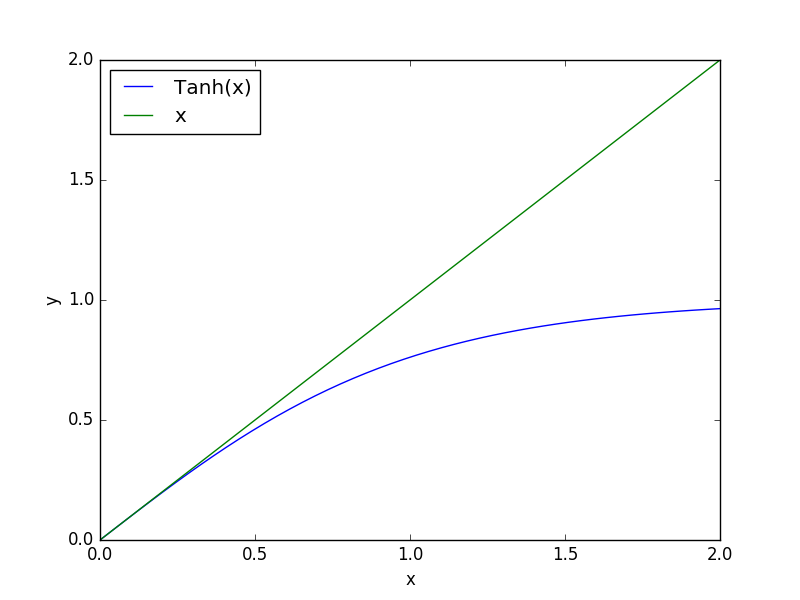
\includegraphics[width=0.8\textwidth]{./Figures/tanh.png}
\end{figure}	
\end{frame}

\begin{frame}{Wave Speed Bounds}
	\begin{equation*}
	v_p = U \pm\sqrt{\frac{g}{k} \tanh\left(kH\right)}
	\end{equation*}	
	\begin{equation*}
	 U - \sqrt{gH} \le v_p \le U +  \sqrt{{g}H}
	\end{equation*}
	\pause
	Limits how fast information can propagate in water	
\end{frame}

\begin{frame}{Shocks}
	Due to bounds on information propagation we observe shocks in water.
	\newline
	Two main examples:
	\begin{itemize}
		\item Bores
		\item Hydraulic Jumps
	\end{itemize}
\end{frame}

\begin{frame}{Bores}
\begin{figure}
	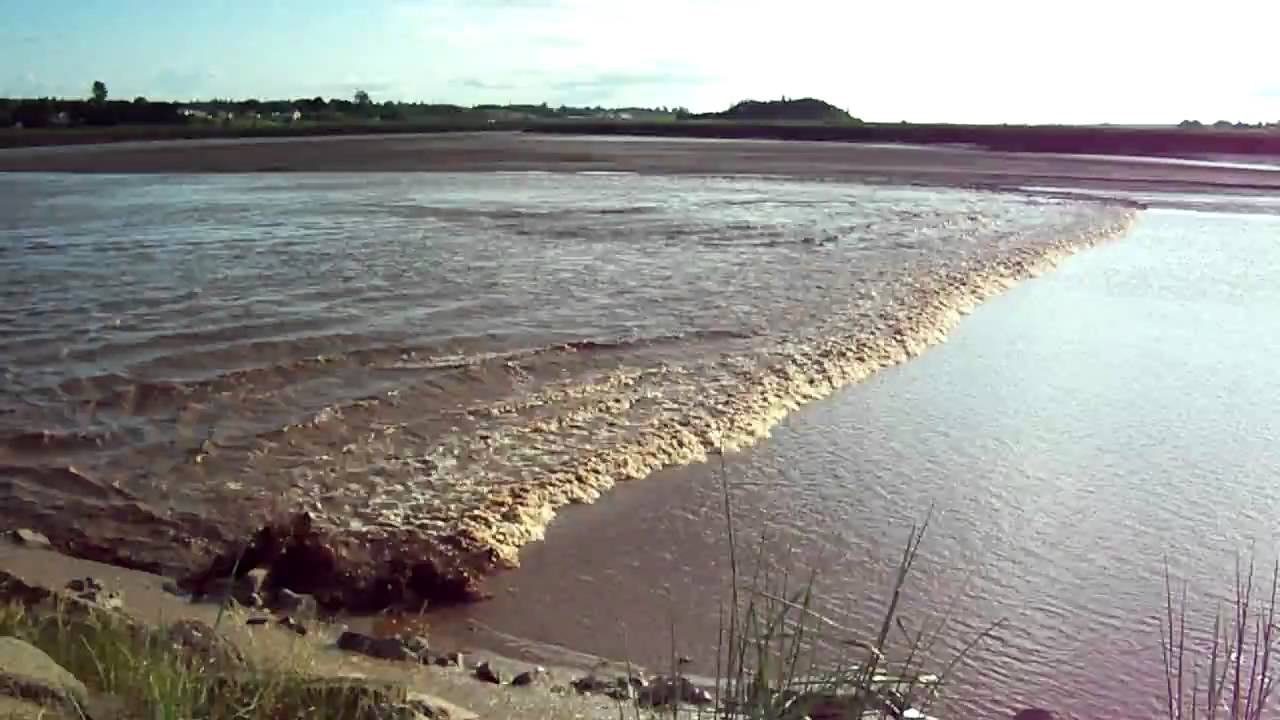
\includegraphics[width=\textwidth]{./Figures/TidalBores.jpg}
	\caption{Tidal Bore (Nova Scotia)}
	%The bores are formed from a combination of effects; funneling estuaries and large tidal differences, 
	%However they propagate as a shock (sudden jump) due to the wave speeds
\end{figure}
\end{frame}

\begin{frame}{Hydraulic Jump}
	\begin{figure}
		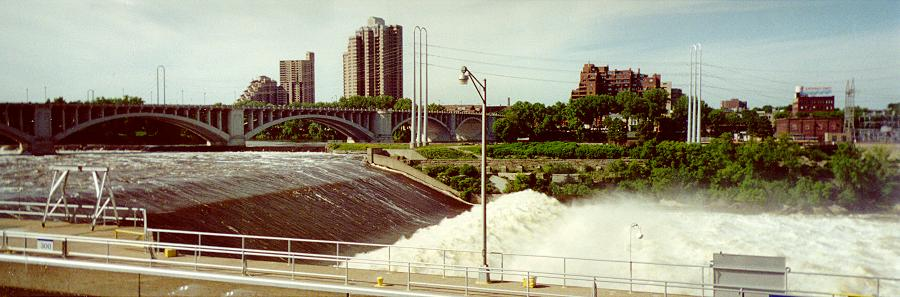
\includegraphics[width=\textwidth]{./Figures/HydrualicJump1.jpg}
		\caption{Hydraulic Jump (Mississippi)}
		%cause by the top of the wave being faster, nonlinearity
		%Sudden decrease
	\end{figure}
\end{frame}

\section{Shallow Water Wave Equations}
\begin{frame}{Shallow Water Wave Equations}
	\begin{subequations}
		\begin{align*}
		&\text{Mass:} && \frac{\partial h}{\partial t} + \dfrac{\partial (uh)}{\partial x} = 0,  \\ \\
		&\text{Momentum:} &&\dfrac{\partial (uh)}{\partial t} + \dfrac{\partial}{\partial x} \left ( u^2h + \dfrac{gh^2}{2} \right )  +  \dfrac{\partial b}{\partial x} \left (gh   \right ) = 0.
		\end{align*}
	\end{subequations}
\end{frame}
\begin{frame}{Characteristics (Wave Speed)}
		$$ v_p = U \pm \sqrt{gH} $$
		So waves in SWWE travel at the fastest possible wave speed in water
		\pause \newline
		Recall for water
		$$ v_p = U \pm\sqrt{\frac{g}{k} \tanh\left(kH\right)}$$
		\pause
		Replacing $\tanh$ with its Taylor series we get
		$$v_p = U \pm \sqrt{gH - \frac{g}{3} H^3 k^2 +  \mathcal{O}\left(k^4H^5\right)}$$
\end{frame}

\begin{frame}{Bore (Dam Break)}
	\begin{figure}
		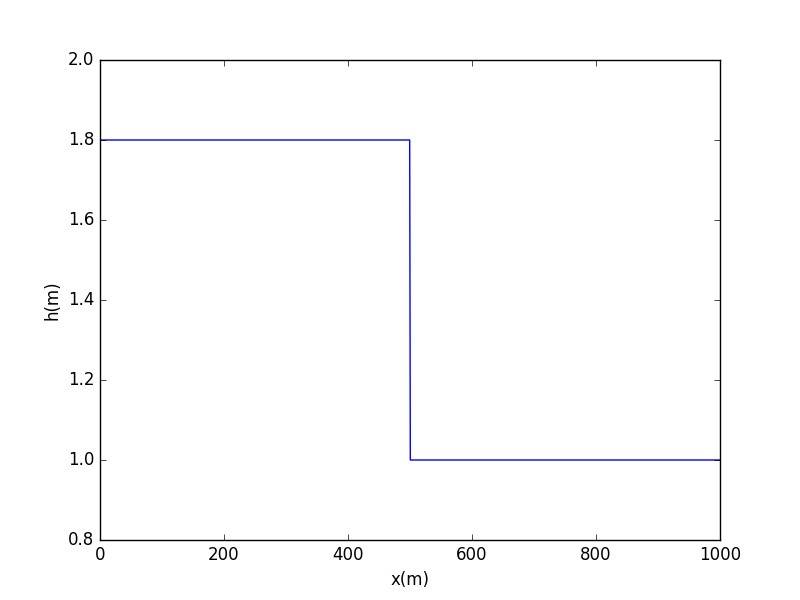
\includegraphics[width=0.7\textwidth]{./Figures/DB.png}
		\caption{Dam-break problem}
	\end{figure}
\end{frame}

\begin{frame}{Bore (Dam Break)}
	\begin{figure}
		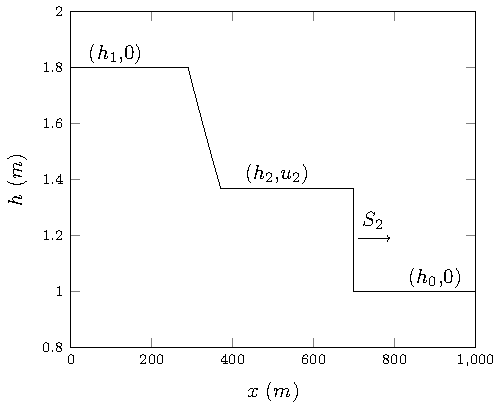
\includegraphics[width=0.7\textwidth]{./Figures/SWWlabel.pdf}
		\caption{Dam-break problem Solution at 30s}
	\end{figure}
\end{frame}

\begin{frame}{Hydraulic Jump}
	\begin{figure}
		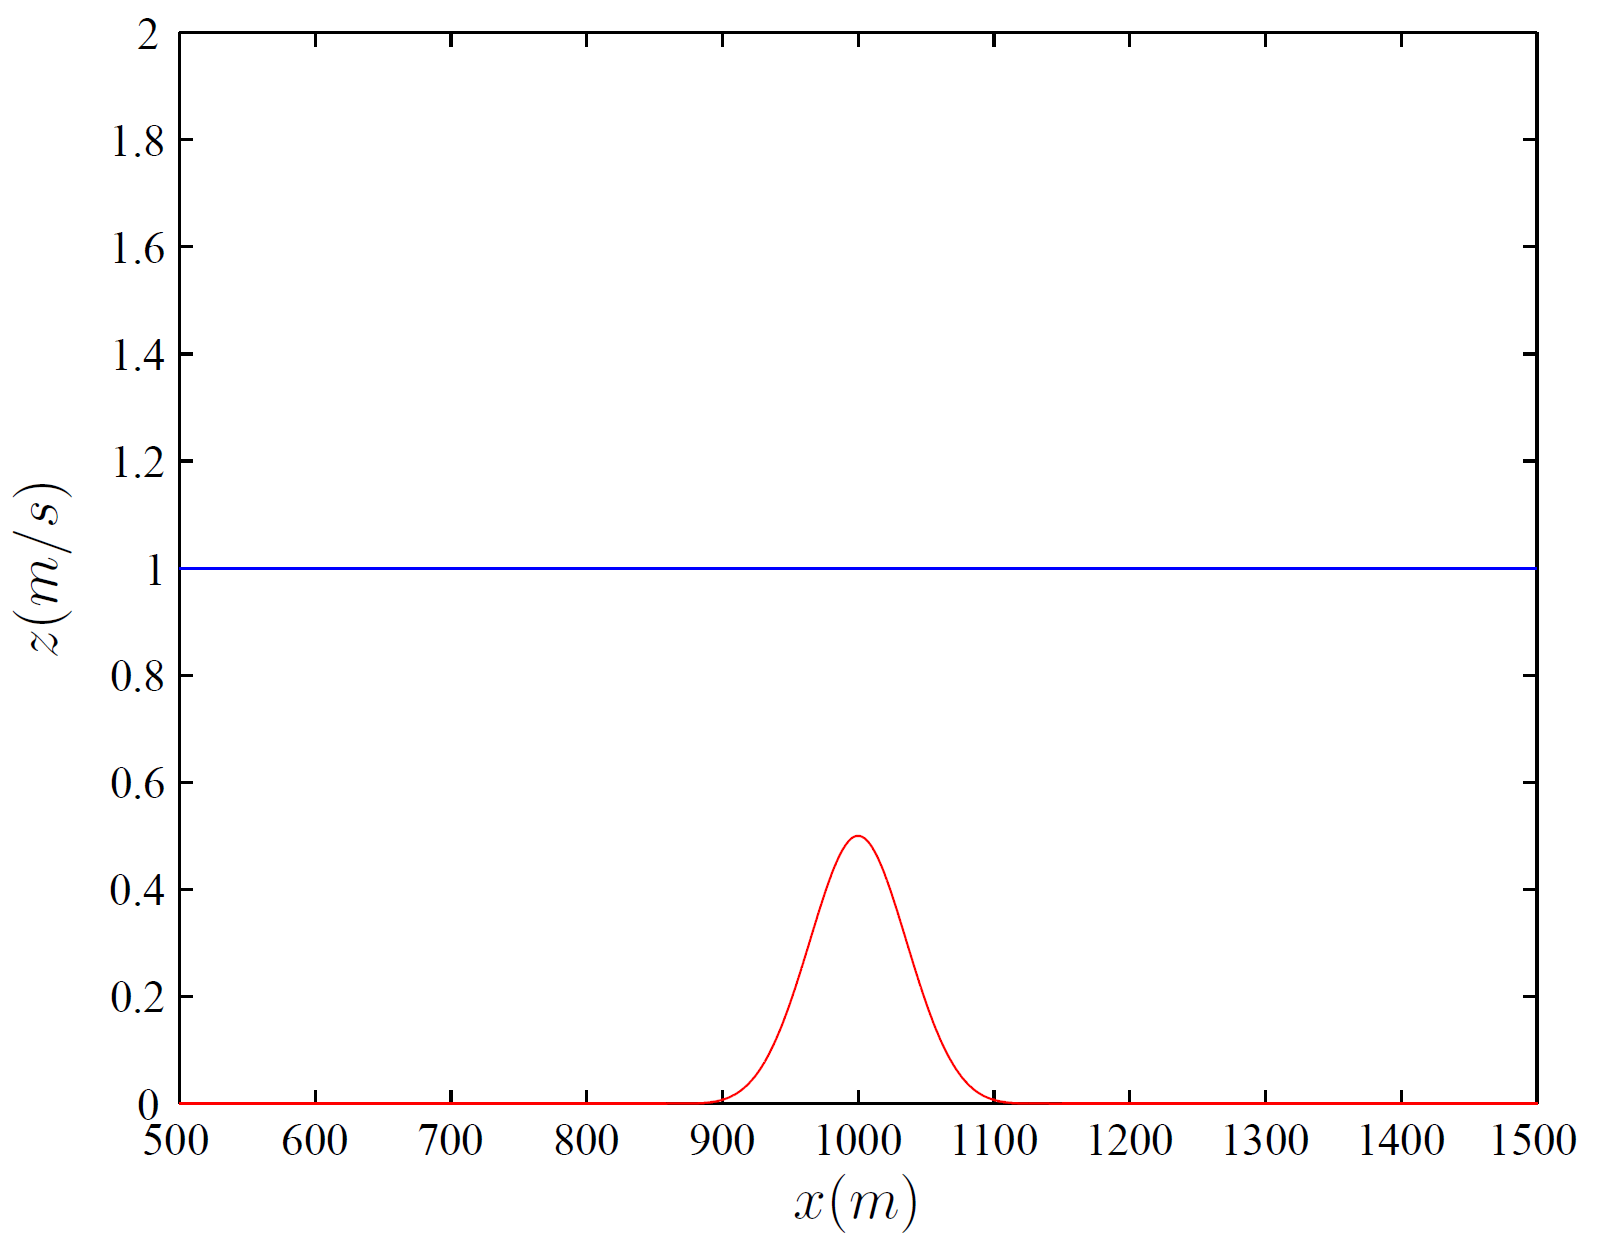
\includegraphics[width=0.7\textwidth]{./Figures/ICu=2.png}
		\caption{Flow over bump $u = 2m/s$ at  $t= 0s$}
	\end{figure}
\end{frame}

\begin{frame}
	\begin{figure}
		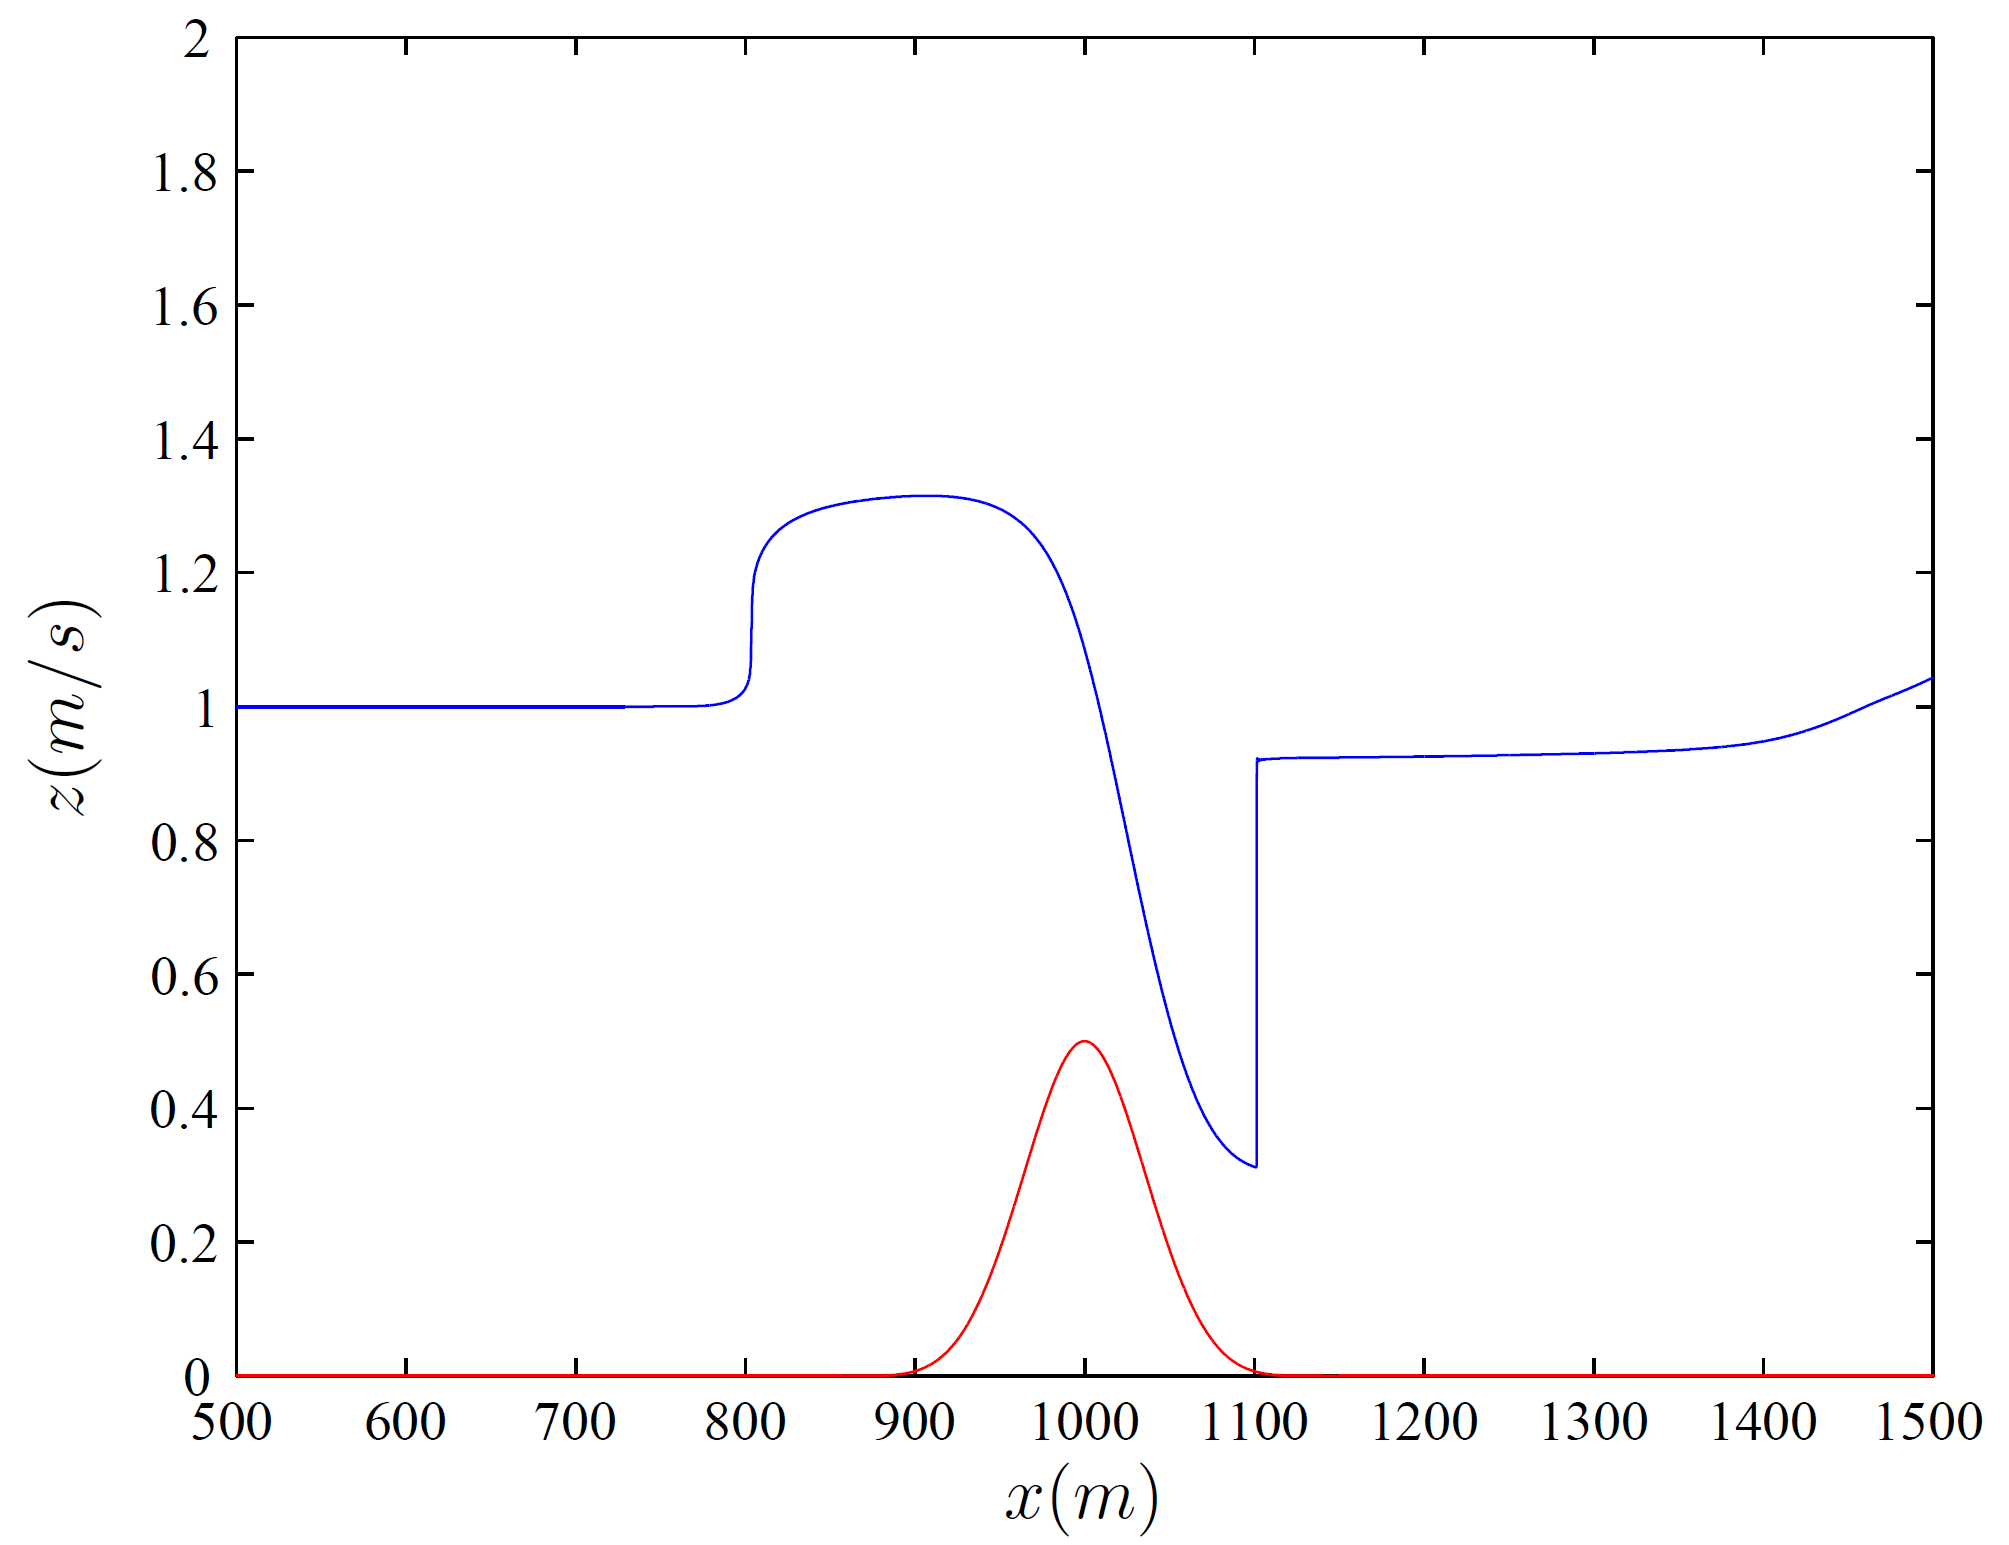
\includegraphics[width=0.7\textwidth]{./Figures/SWWEt=100s.png}
		\caption{Flow over bump at $t= 100s$}
	\end{figure}
\end{frame}

\begin{frame}
	\begin{figure}
		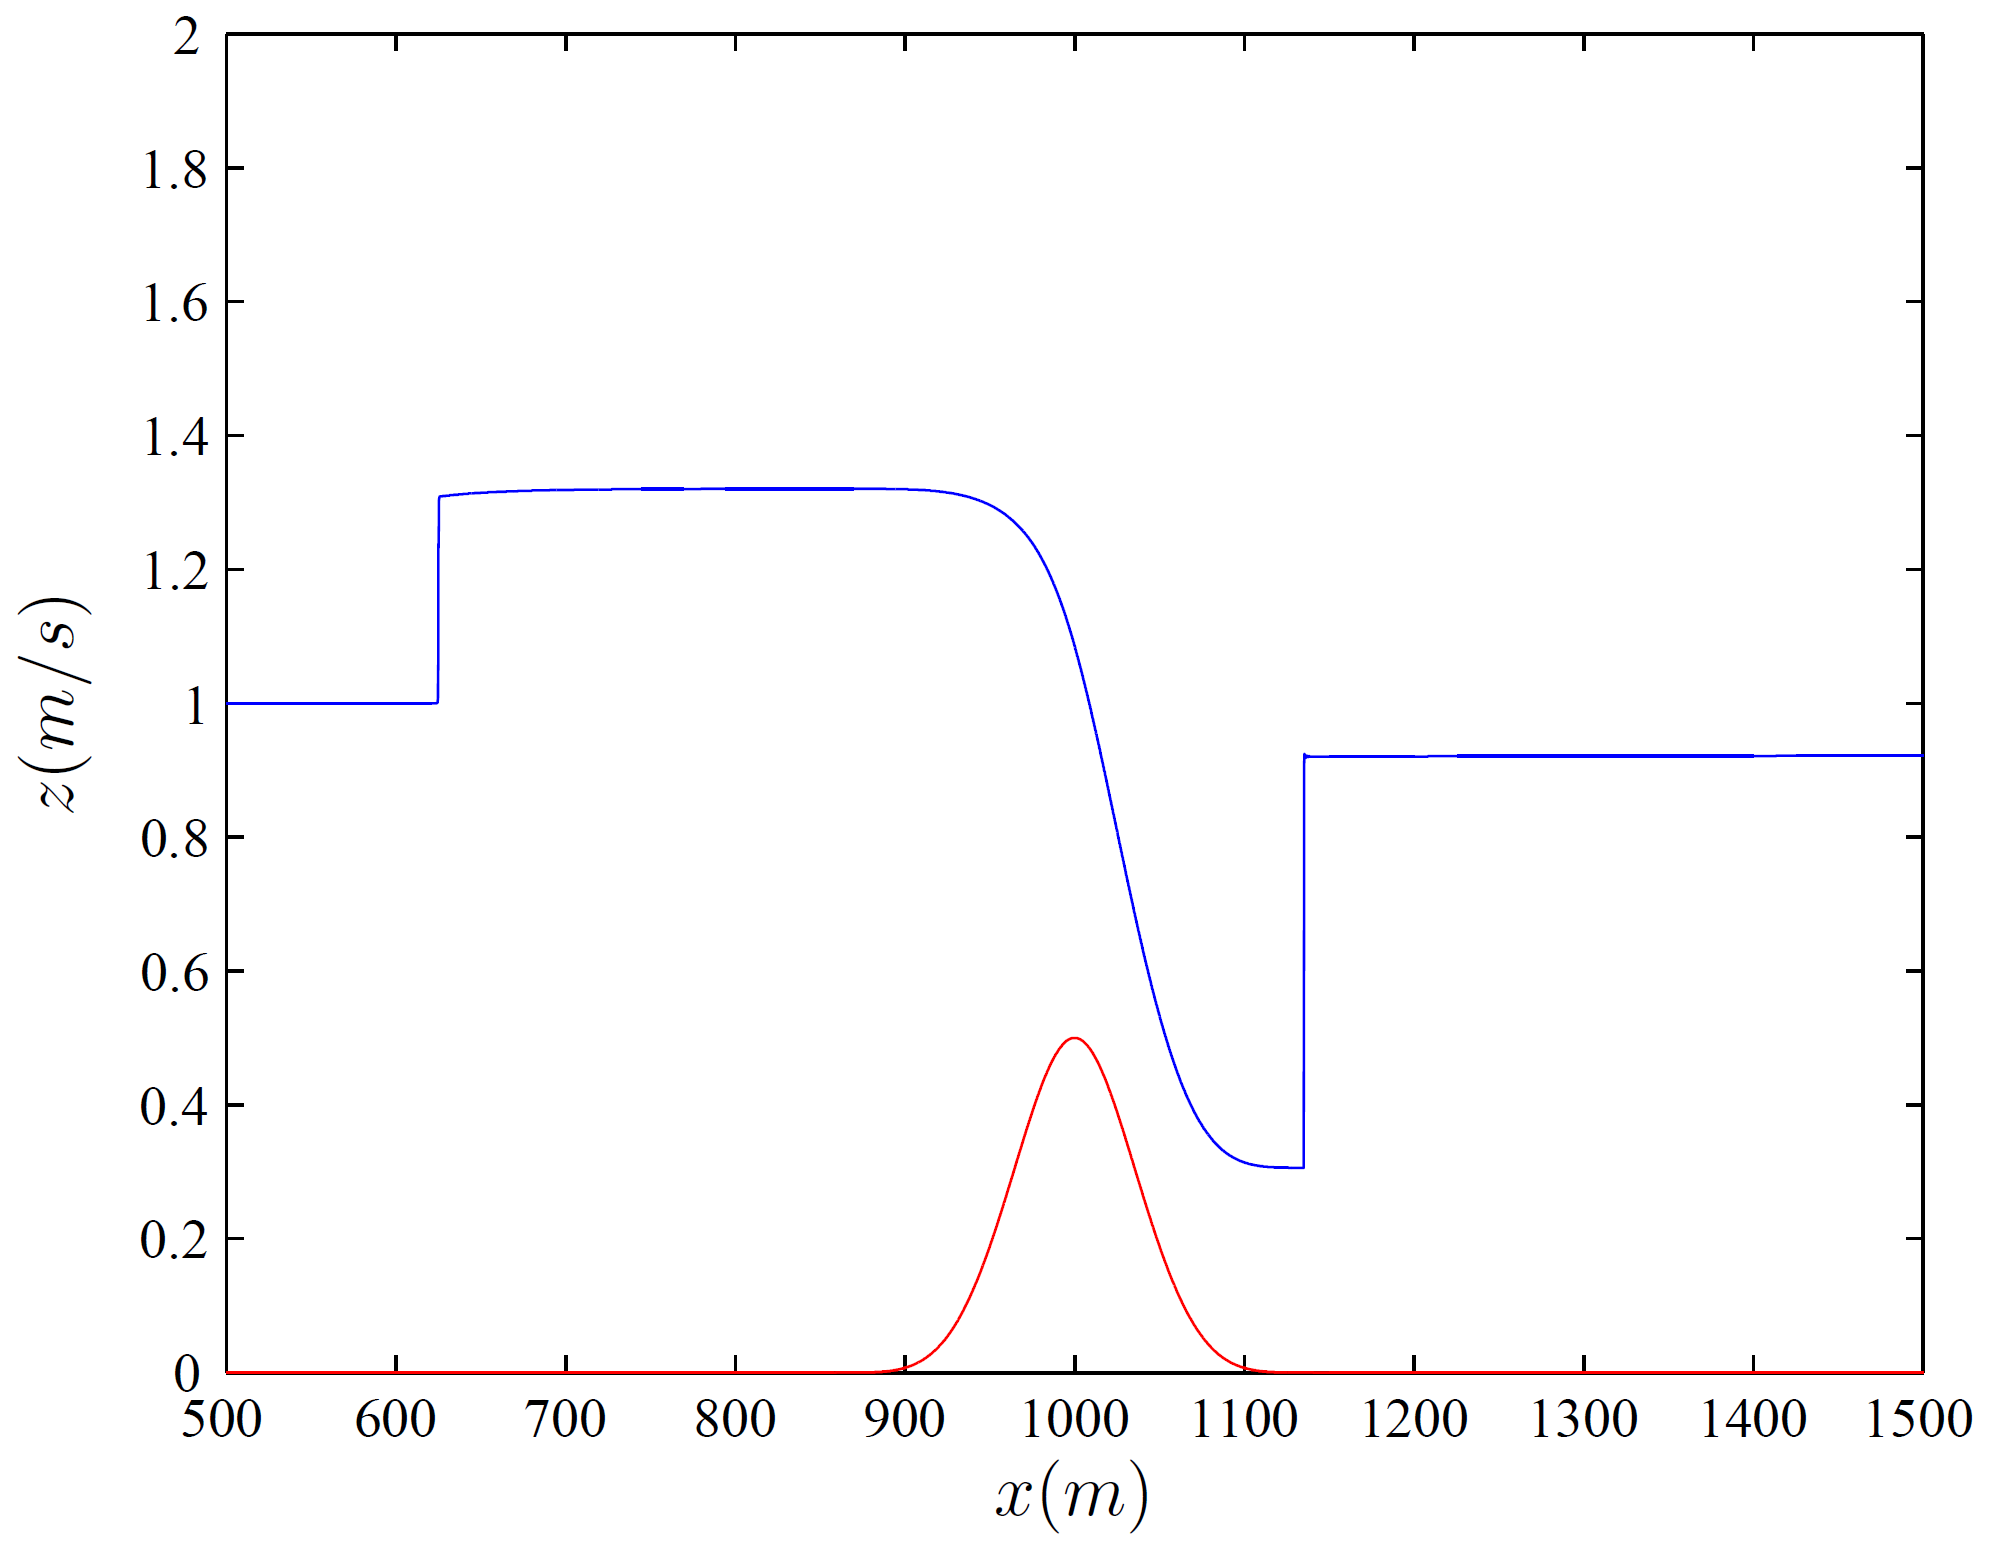
\includegraphics[width=0.7\textwidth]{./Figures/SWWEt=200s.png}
		\caption{Flow over bump at $t= 200s$}
	\end{figure}
\end{frame}

\begin{frame}
	\begin{figure}
		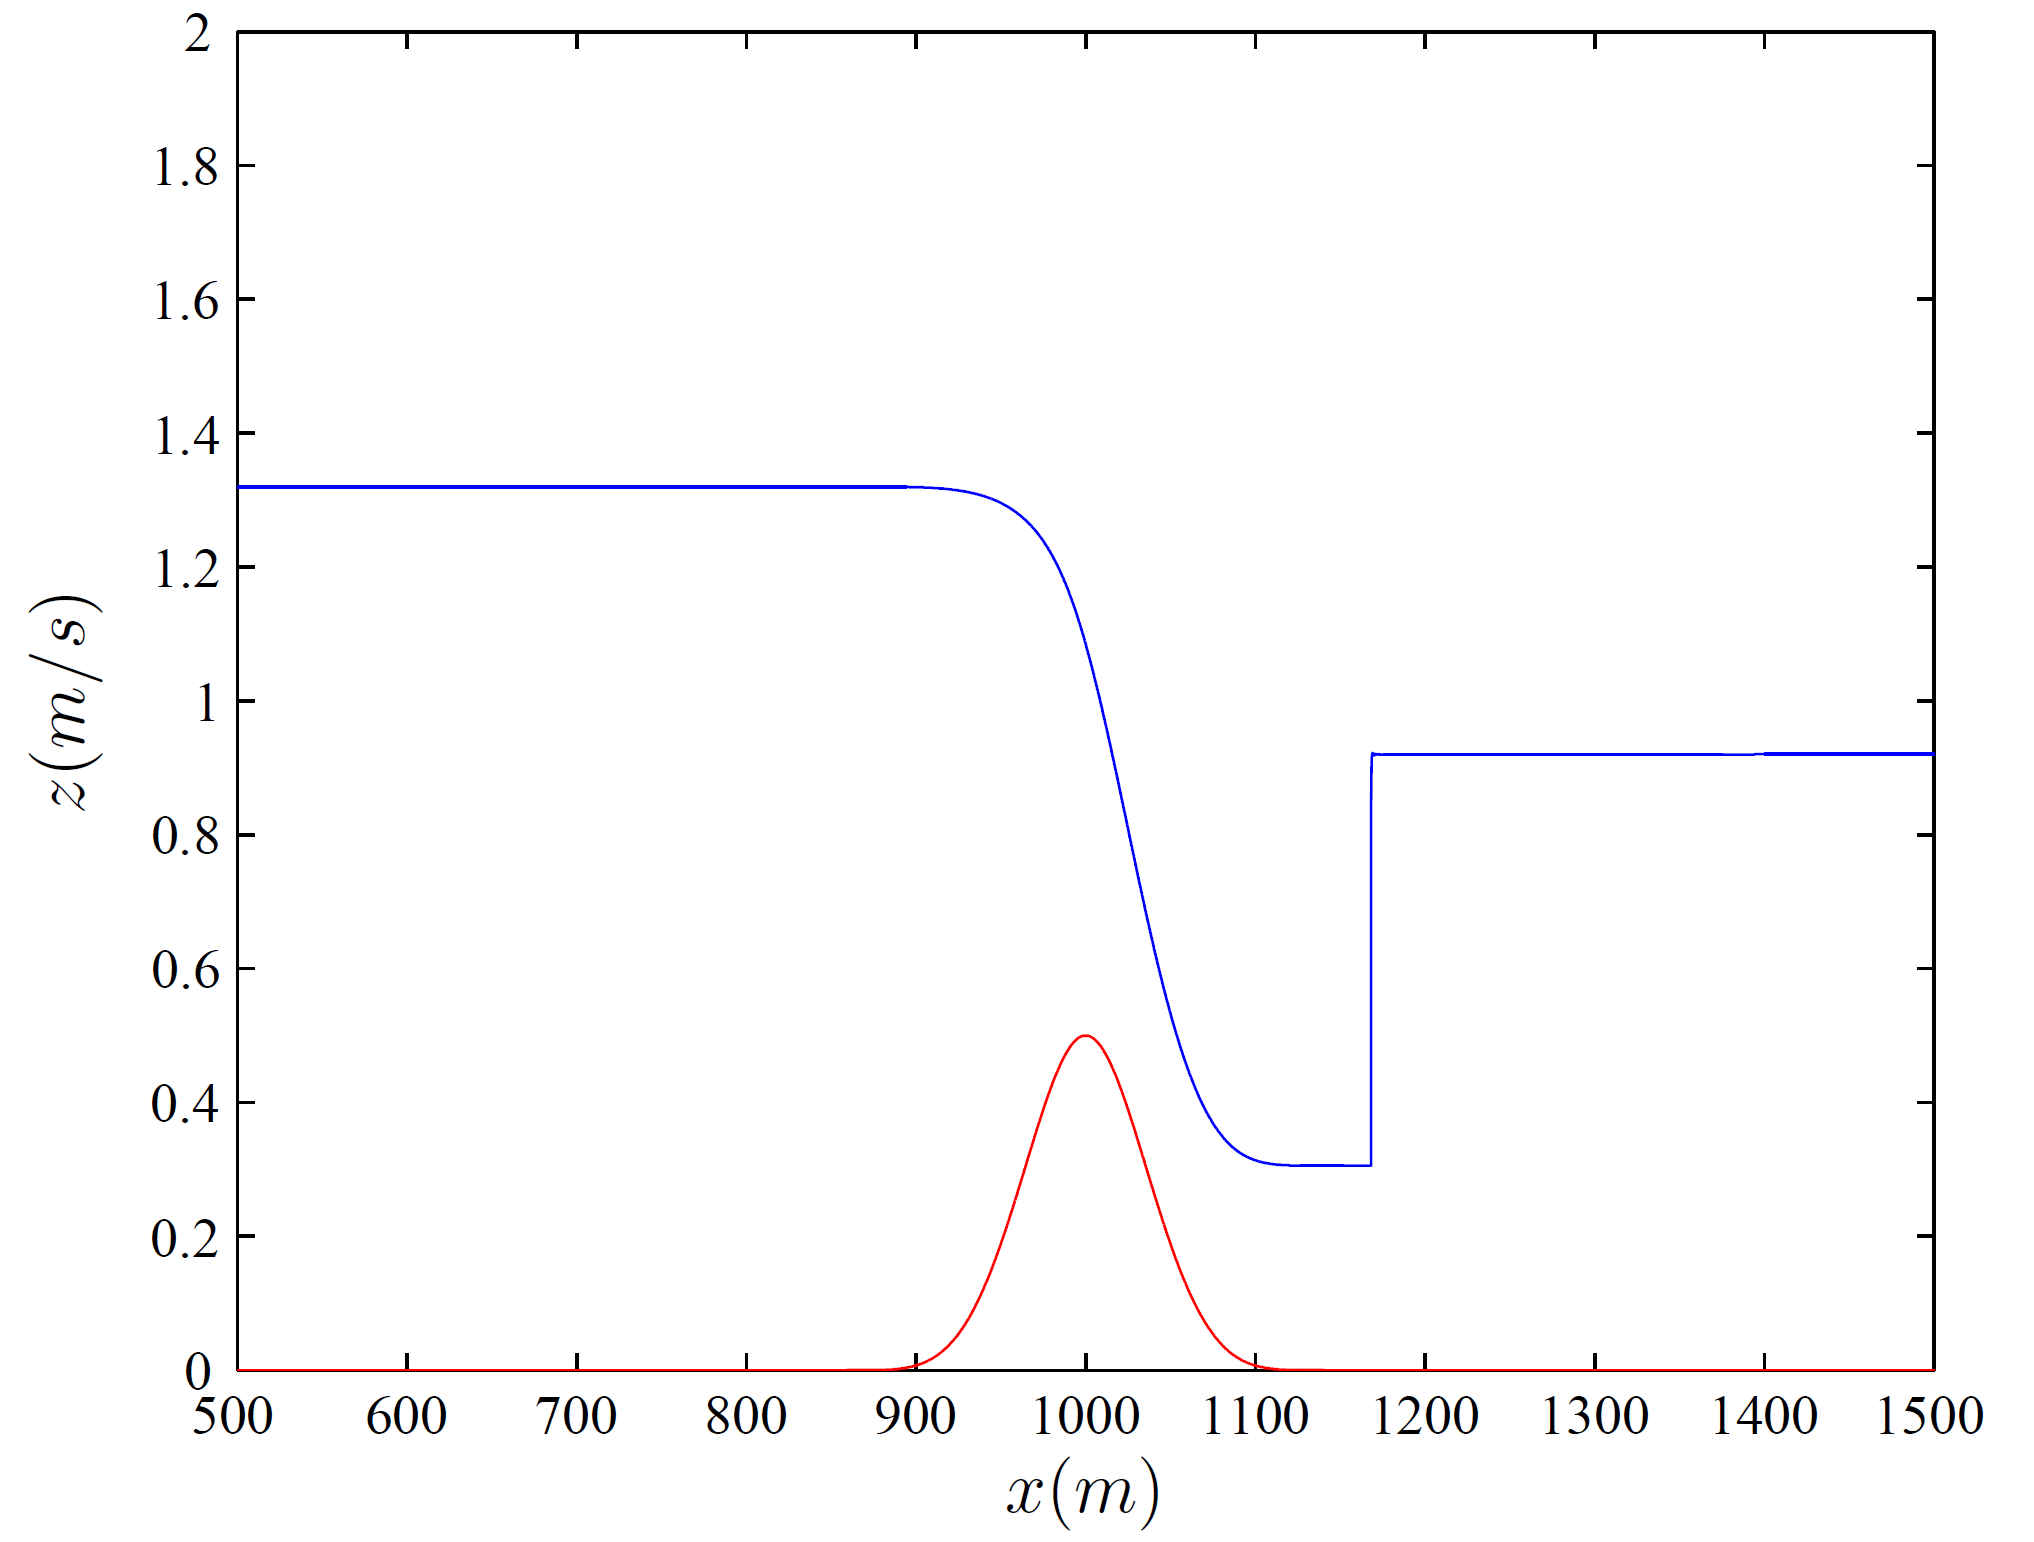
\includegraphics[width=0.7\textwidth]{./Figures/SWWEt=300s.png}
		\caption{Flow over bump at $t= 300s$}
	\end{figure}
\end{frame}


\section{Serre Equations}
\begin{frame}{Serre Equations}
	\begin{subequations}
		\begin{align*}
		&\text{Mass:} && \frac{\partial h}{\partial t} + \dfrac{\partial (uh)}{\partial x} = 0,  \\ \\
		&\text{Momentum:} &&\dfrac{\partial (uh)}{\partial t} + \dfrac{\partial}{\partial x} \left ( u^2h + \dfrac{gh^2}{2} + \dfrac{h^2}{2}{ \color{red}\Psi } + \dfrac{h^3}{3}{ { \color{blue} \Phi } }  \right )   \\ \\& &&\quad \quad \; \; +  \dfrac{\partial b}{\partial x} \left (gh +   h { \color{red}\Psi } + \dfrac{h^2}{2}{ { \color{blue} \Phi } }  \right ) = 0.
		\end{align*}
	\end{subequations}
	\begin{align*}
	&{ \color{red}\Psi }  = \dfrac{\partial b}{\partial x}\left(\dfrac{\partial u}{\partial t} + u\dfrac{\partial u}{\partial x} \right)  + u^2\dfrac{\partial^2 b}{\partial x^2}, &
	{ \color{blue} \Phi }  = \dfrac{\partial u }{\partial x} \dfrac{\partial u}{\partial x} -u \dfrac{\partial^2 u}{\partial x^2}  - \dfrac{\partial^2 u}{\partial x \partial t} .
	\end{align*}
\end{frame}

\begin{frame}{Wave Speeds}
	$$ v_p = U \pm \sqrt{gH} \sqrt{\frac{3}{k^2 H^2 +3}} $$
	\pause
	Taylor series of this is
	$$v_p = U \pm \sqrt{gH - \frac{g}{3} H^3 k^2 +  \mathcal{O}\left(k^4H^5\right)}$$
	\pause \newline
	Recall for water the Taylor series was
	$$v_p = U \pm \sqrt{gH - \frac{g}{3} H^3 k^2 +  \mathcal{O}\left(k^4H^5\right)}$$
\end{frame}

\begin{frame}{Result}
	Not only do we get the shocks due to the bounds on the wave speeds but we also get some of that internal structure we see in the real world
\end{frame}

\begin{frame}{Dam Break}
	\begin{figure}
		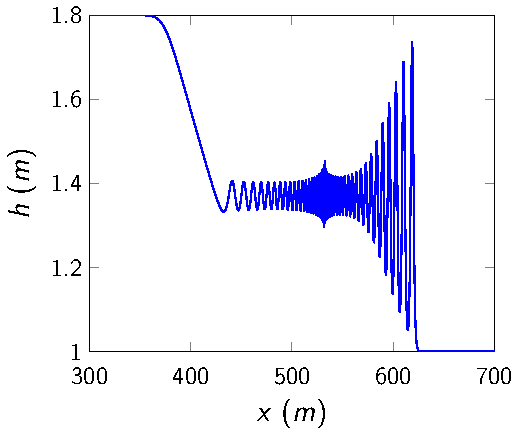
\includegraphics[width=0.6\textwidth]{./Figures/h3.pdf}
		\caption{Dam-break problem solution at 30s}
	\end{figure}
\end{frame}

\begin{frame}{Wave Speed Effects}
	$$ v_p = U \pm \sqrt{gH} \sqrt{\frac{3}{k^2 H^2 +3}} $$
	\pause
	$$ v_p^- =  U - \sqrt{gH}\sqrt{\frac{3}{k^2 H^2 +3}} \le U \le  U +\sqrt{gH}\sqrt{\frac{3}{k^2 H^2 +3}} = v_p^+ $$
\end{frame}

\begin{frame}{Evolution}
	\begin{figure}[ht]
		\includemovie[
		poster,
		text={}
		]{6cm}{6cm}{./Figures/CDs.mp4}
	\end{figure}
\end{frame}

\begin{frame}{Hydraulic Jump}
	\begin{figure}
		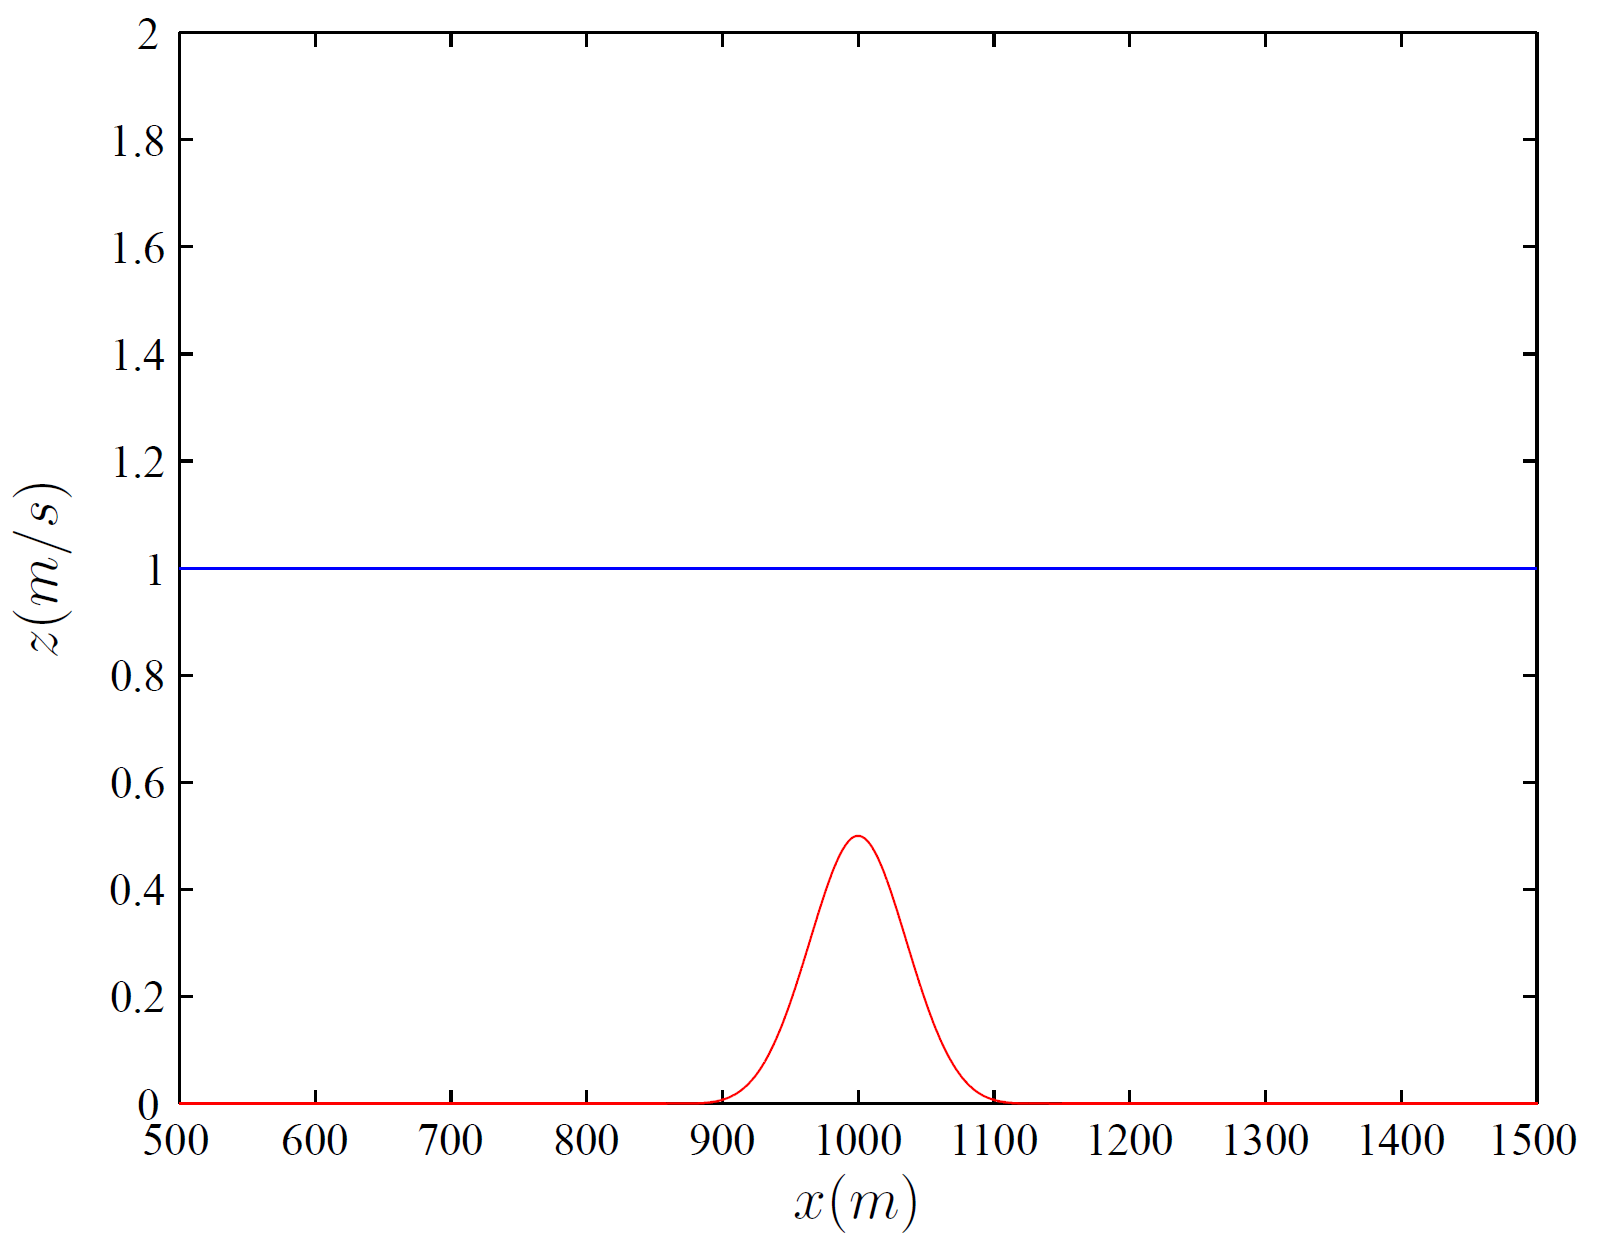
\includegraphics[width=0.7\textwidth]{./Figures/ICu=2.png}
		\caption{Flow over bump $u = 2m/s$ at  $t= 0s$}
	\end{figure}
\end{frame}

\begin{frame}
	\begin{figure}
		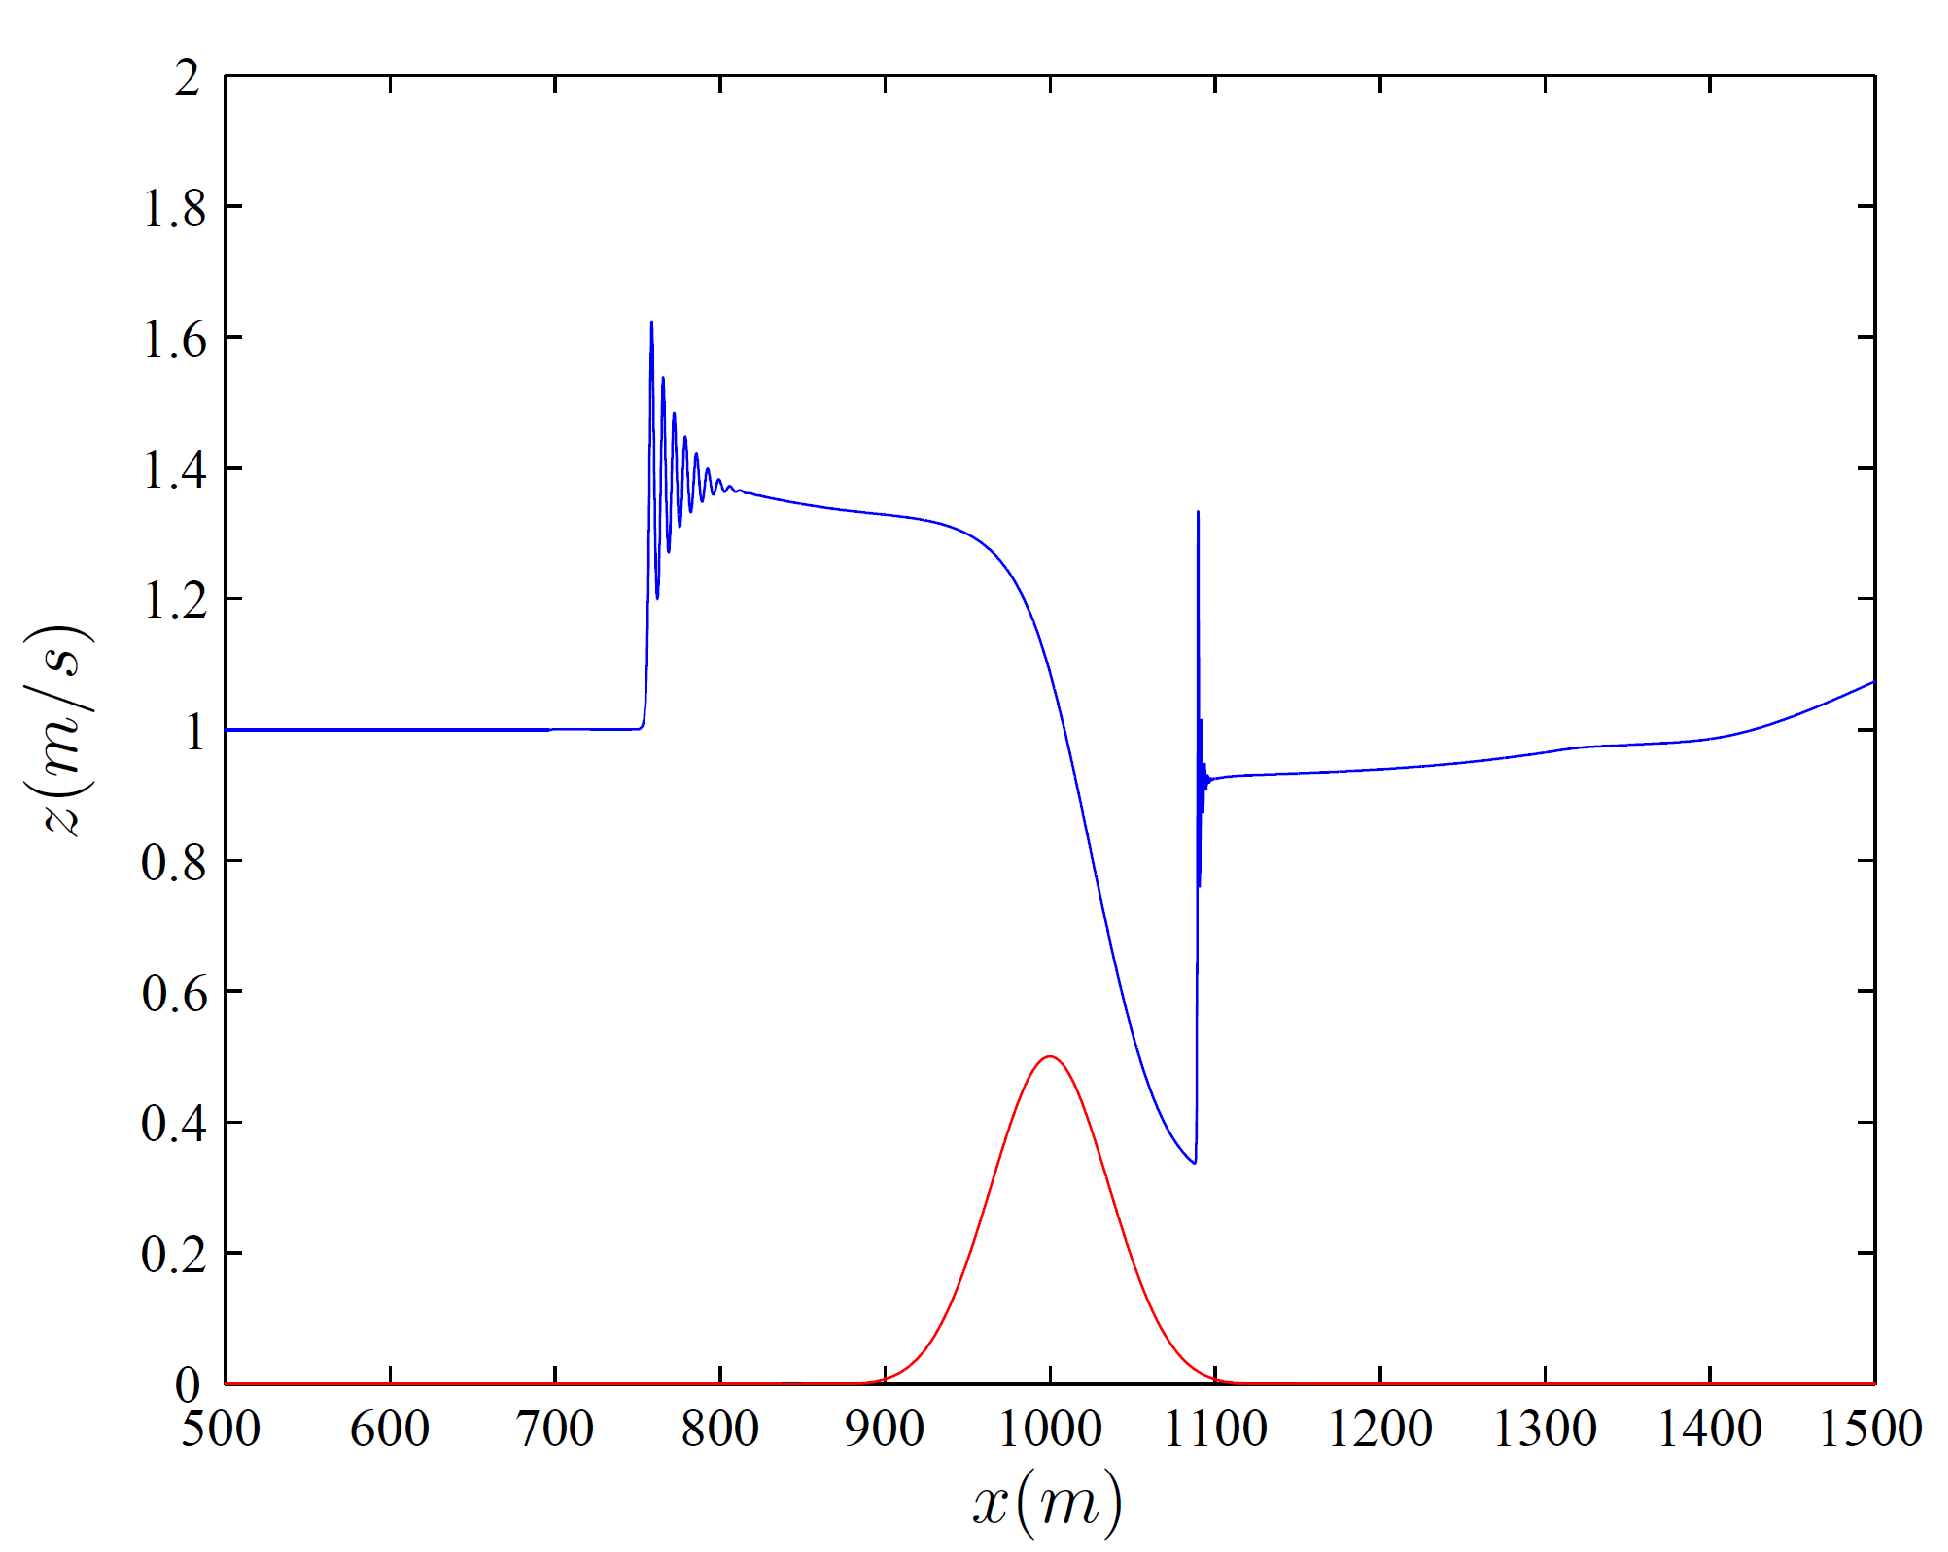
\includegraphics[width=0.7\textwidth]{./Figures/Serret=100s.png}
		\caption{Flow over bump at $t= 100s$}
	\end{figure}
\end{frame}

\begin{frame}
	\begin{figure}
		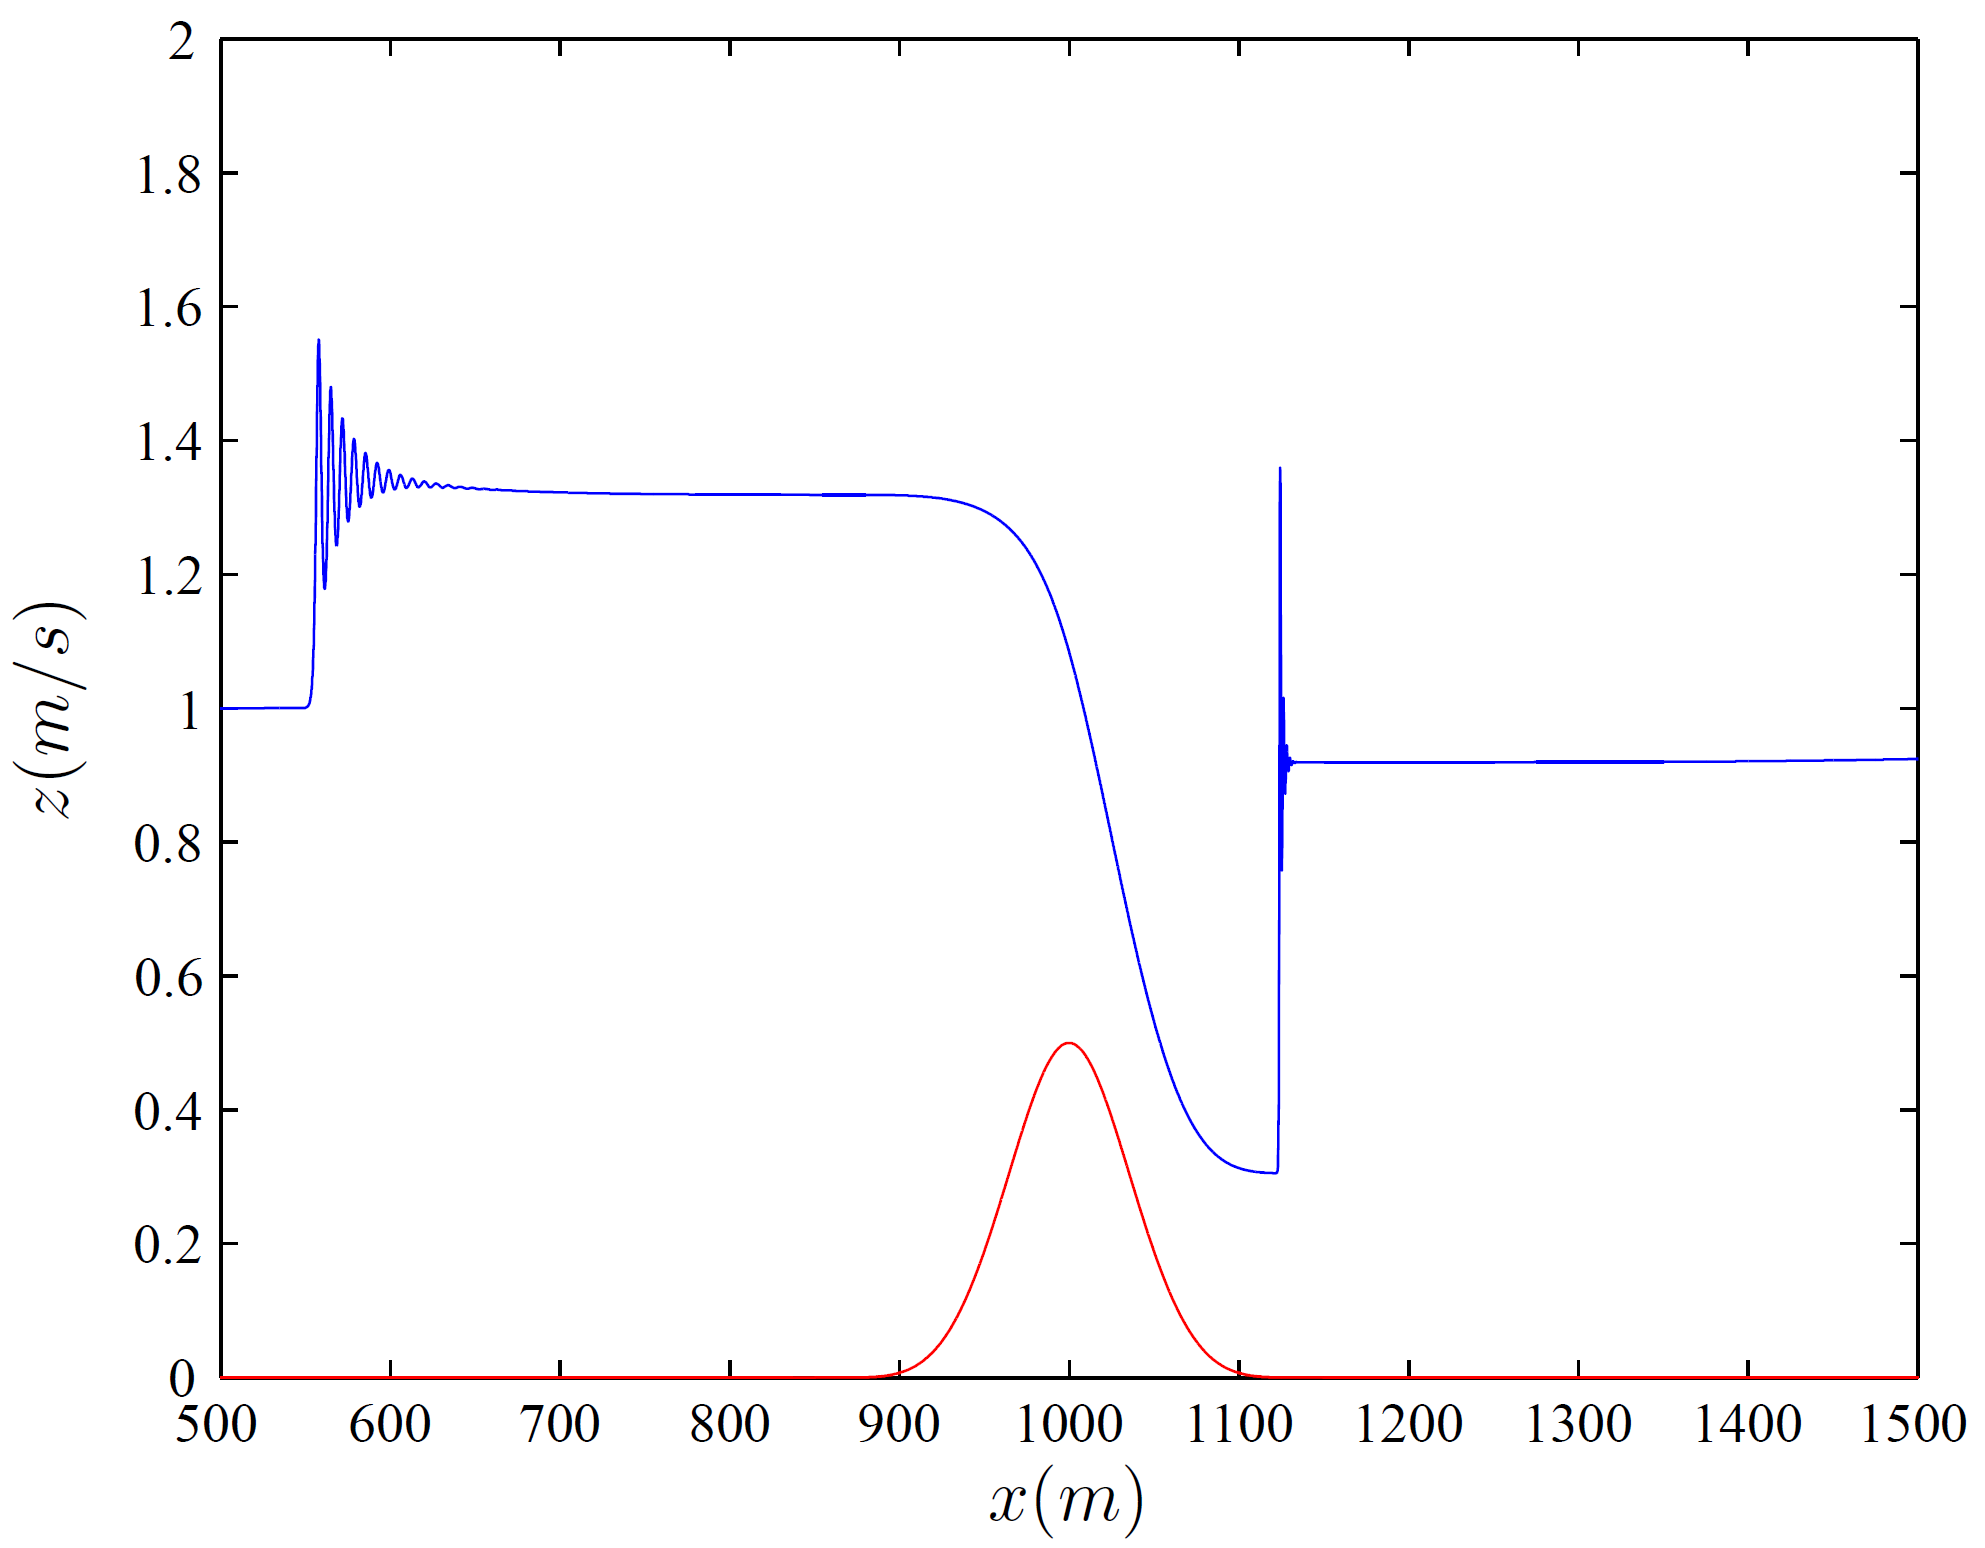
\includegraphics[width=0.7\textwidth]{./Figures/Serret=200s.png}
		\caption{Flow over bump at $t= 200s$}
	\end{figure}
\end{frame}

\begin{frame}
	\begin{figure}
		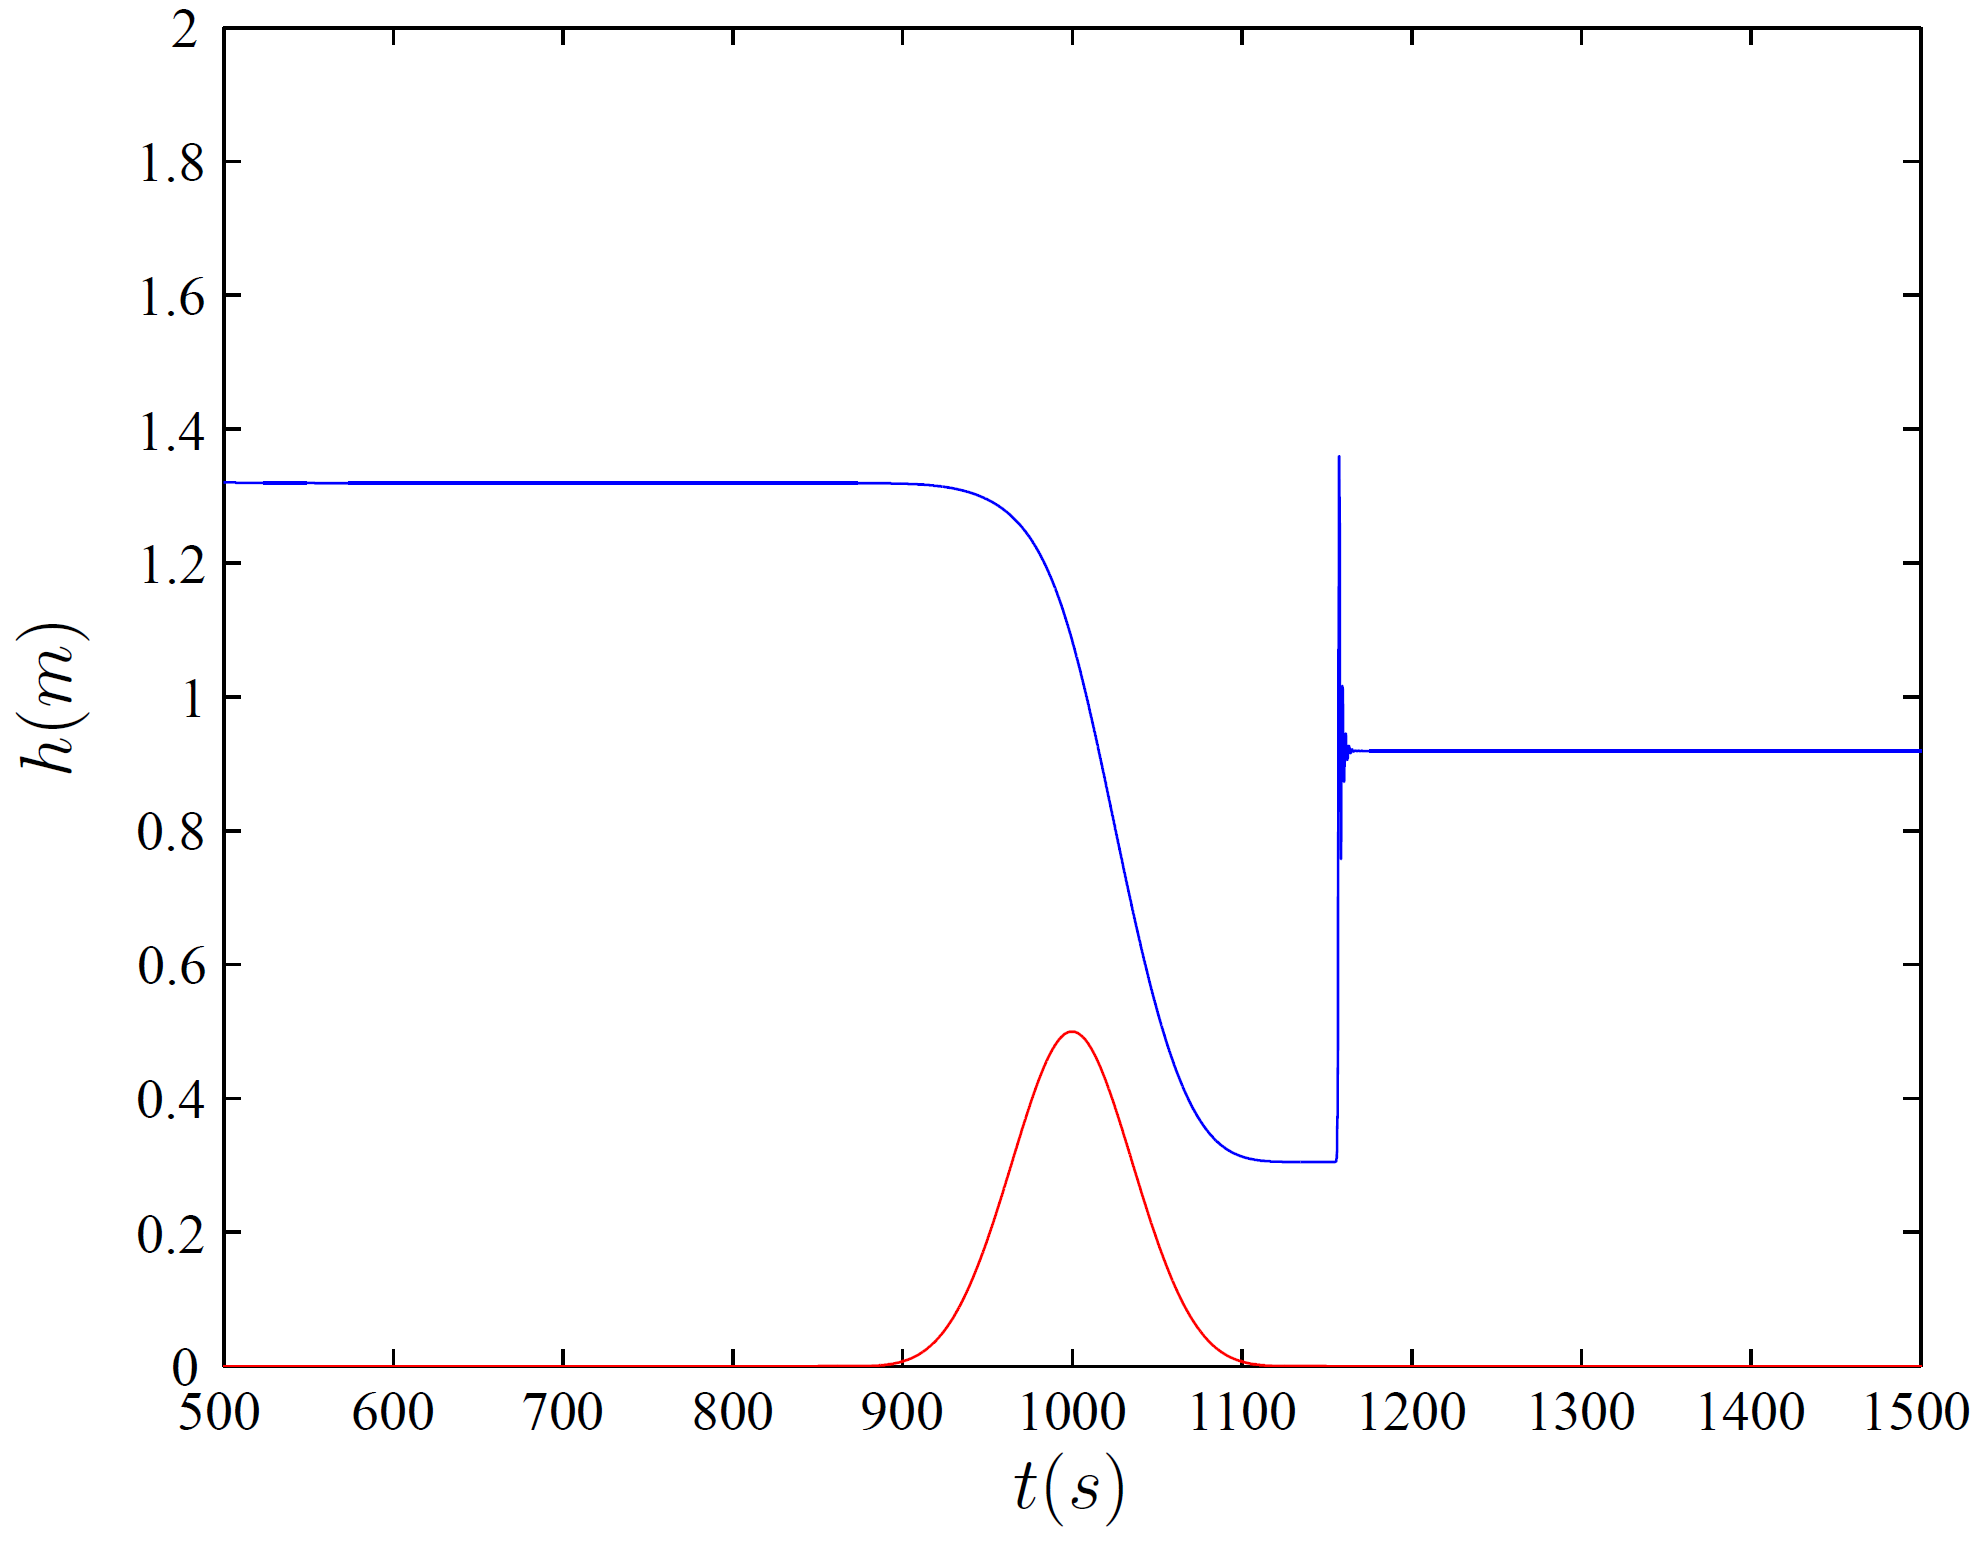
\includegraphics[width=0.7\textwidth]{./Figures/Serret=300s.png}
		\caption{Flow over bump at $t= 300s$}
	\end{figure}
\end{frame}

\end{document}